\documentclass[oneside,12pt]{amsart}
\usepackage[english]{babel}
\usepackage{graphicx}
\usepackage{float}
\usepackage{mathtools}
\usepackage{amsfonts}
\usepackage{amssymb}
\usepackage{siunitx}
\usepackage{amsthm}
\usepackage{enumitem}
\usepackage{stmaryrd}
\usepackage{multirow}
\usepackage[backend=bibtex,style=numeric]{biblatex}
\bibliography{Biblio}
\usepackage[a4paper, total={6in, 10in}]{geometry}
\graphicspath{{./}{}}% You can add the path for the images in the empty brackets 
\title{Study of Electrostatics: Generation and Measurement of Charge}
\author{Josh Goldfaden, Daniel Briseno}
\date{}
\newdimen\graph
\graph=4.2in
\newdimen\medgraph
\medgraph = 5.3in
\newdimen\smallgraph
\smallgraph = 3in
\newdimen\tinygraph
\tinygraph = 1.5in
\renewcommand{\arraystretch}{1.5}
\begin{document}
	\maketitle
	\section{Abstract}
	\indent In this set of experiments, the electric potential at various locations on a semi-conductive grid paper that was coded with conductive silver ink was mapped using a Vernier Power Amplifier integrated with a computer. However, the results of the experiment were inconclusive since we found that the semi-conductive paper was faulty, and acted as a conductor nearly throughout the entire paper.
	\section{Introduction}
	Potential Energy exists both within macroscopic objects that are studied in classical mechanics as well as in quantum objects. Regarding potential energy in the latter, charged particle will exert a force on any neighboring charged particles. Inevitably, in such an arrangement of charges, potential energy also exists. For instance, if a positively charged particle Q is stationary within a given area, any other positive charge particles brought within a close vicinity of particle Q will create a repulsive force and will thus generate a potential energy. Below is a visual representation of particle Q at a distance r from a test charge q\cite{electricpotentialenergy}:
	\begin{figure}[H]
		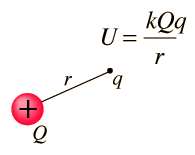
\includegraphics[width=\smallgraph,scale=0.01]{Pontential.png}
		%h (here) - same location
		%t (top) - top of page
		%b (bottom) - bottom of page
		%p (page) - on an extra page5
		%! (override) - will force the specified location
		\caption{ Visual representation of particle Q at a distance r from a test charge q  \cite{electricpotentialenergy}}
		\label{Potential}
	\end{figure}
	
	\indent Mathematically, electric potential energy can be expressed by the following equation:
	\begin{align}
		U &= \frac{kQq}{r}
	\end{align}
	where k is Coulomb’s constant, Q is the charge of the particle, q is the test charge, and r is the distance between the test charge and the charged particle. It is also noteworthy that the units of potential energy are expressed as the product of coulombs and volts squared divided by two (CV2/2). 
	
	\section{Plotting Electric Potential}
		In this experiment, we wanted to produce a map of electric potential at various locations on a semi-conductive grid paper that is covered with conductive silver ink. This sheet of paper was pinned at the points of the painted electrodes using conductive pushpins. Then, the clip leads originating from the terminal of a Vernier Power Amplifier were connected to the pushpins. We then measured the electric potential throughout the paper and constructed the 2-d topological map shown in figure \ref{2d}.\\
		
		\begin{figure}[h]
		 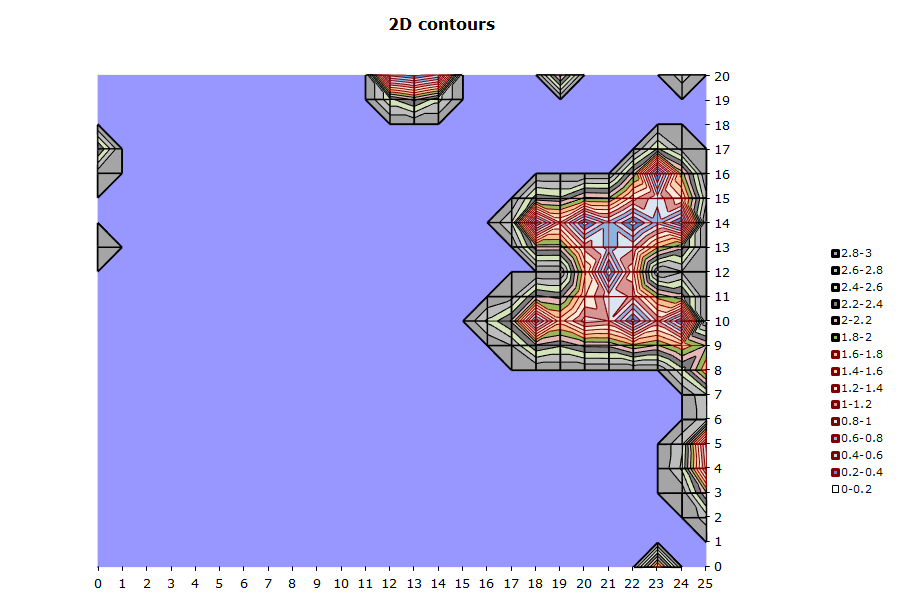
\includegraphics[width=\smallgraph,scale=0.01]{2d.png}
		\caption{Graph showing results of defective semi-conductor paper.}
		\label{2d}
		\end{figure}
	
		\begin{figure}[h]
		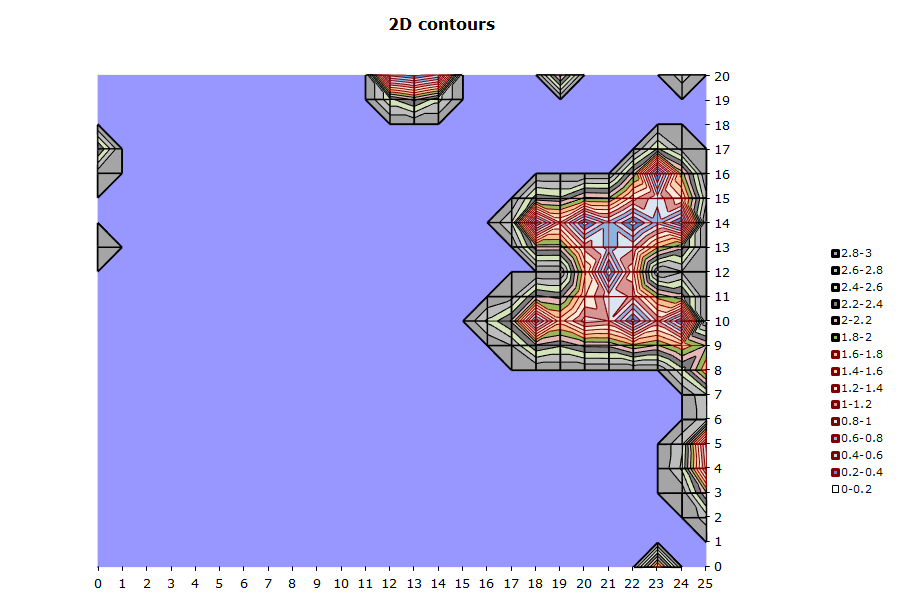
\includegraphics[width=\smallgraph,scale=0.01]{image.png}
		\caption{Graph showing results of defective semi-conductor paper.}
		\label{3d}
	\end{figure}
	
		\indent As seen in figures \ref{2d}, \ref{3d}, the data we collected yielded a topological map that shows a nearly uniform electric potential. This leads us to the conclusion that the paper we used was defective, since it seemed to act as a conductor rather than a semi-conductor along most of its area.\\
		
		\indent What we \textit{expected} to have seen is circular equipotential lines extending from the circular silver ink electrode and the negative terminal. We would have expected that the lines would have been very dense near the electrodes, and would have spaced out as the distance from any electrode increased. Lastly, we would have expected the equipotential lines to ``flatten out" between the two particles.\\
		
		\indent Since we know that the strength of the electric field must be strongest near a charge and weaken as we move away from the charge, we can see that the spacing of the equipotential lines at a point (or in a 3-d topological map, the steepness of the equipotential surface) is indicative of the strength of the electric field at that point. Knowing that electric field lines should be perpendicular to the equipotential lines, we can determine the electric field generated by a charged object given information about the electric potentials around the object. 
		\begin{figure}[h]
			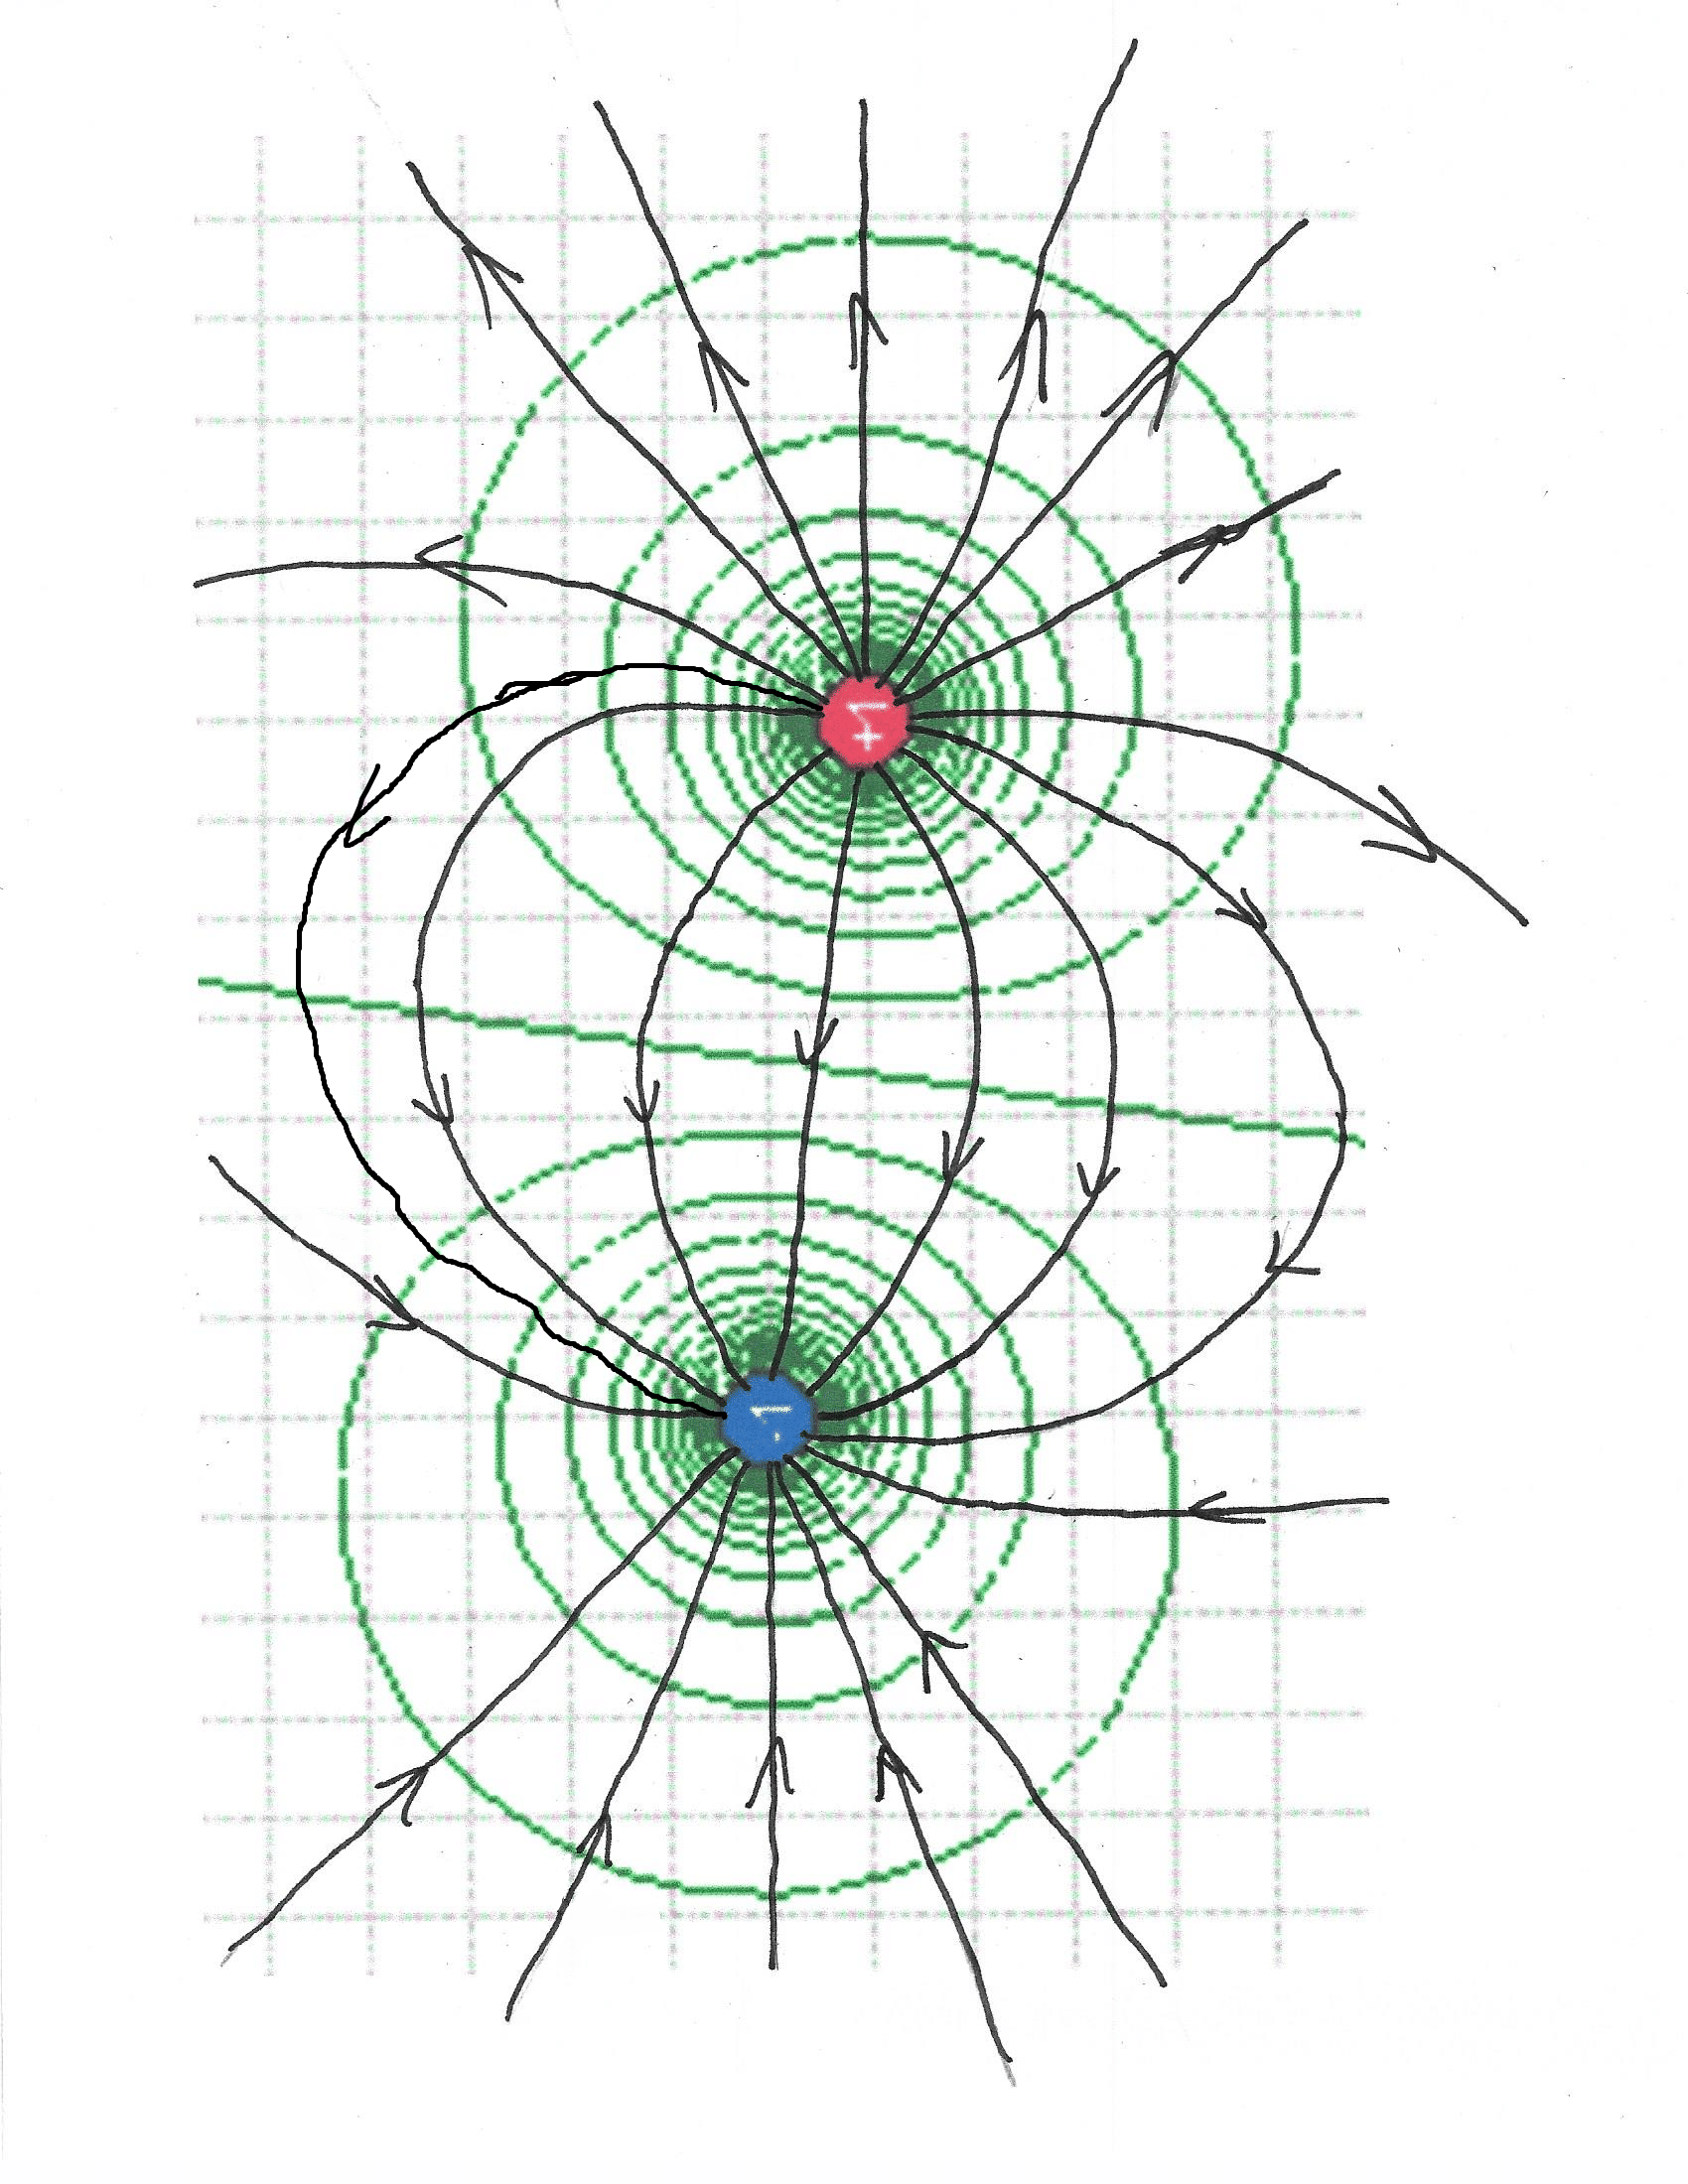
\includegraphics[width=\smallgraph,scale=0.01]{field1.png}
			%h (here) - same location
			%t (top) - top of page
			%b (bottom) - bottom of page
			%p (page) - on an extra page5
			%! (override) - will force the specified location
			\caption{Electric Field outlined by equipotential topology. Electric potential graph taken from \cite{field}}
			\label{field}
		\end{figure}
	
	\section{Conclusion}
	Although we intended to measure the electric potential generated by the two electrodes on the semi-conducting paper, we quickly saw that the paper was defective and giving a nearly constant potential at all points. However, using a map of electric potentials taken from an outside source \cite{field}, we were still able to see how the shape and magnitude of an electric field can be determined by electric potentials.
		
		\newpage
		\printbibliography
\end{document}